\chapter{Desarrollo}

El sistema IoT propuesto para una habitación de un entorno Smart House representado por el esquema de la Figura \ref{fig:diagramas}, pretende ser fácil de visualizar y manipular por el usuario, por este motivo se desarrolla una aplicación web (software) que permite la cómoda navegación a través de ella y que las interacciones humano-máquina sean de manera intuitiva. Esta característica del sistema está diseñada de tal manera que solo los usuarios puedan ver el estado de la habitación, ya que para hacerlo es necesario ingresar las credenciales oficiales otorgadas por el Usuario Administrador, el cual es uno de los tres roles de usuario existentes en el sistema, junto con el rol de Usuario Casa y Usuario Habitación.\\

Como se mencionó anteriormente, el Usuario Administrador es quien otorga las credenciales a los demás usuarios, ya que este tiene la facultad de crear, editar y eliminar los registros de la aplicación, lo cual a su vez lo hace exclusivo, es decir, no esta abierto para el público o los clientes.\\ 

En ese orden de ideas, los demás usuarios tienen privilegios limitados a las necesidades de cada rol, es decir, los Usuarios Casa tienen acceso a la revisión y edición de algunos campos de las viviendas registradas a su nombre y de los usuarios Habitación vinculados a él, además de poder gestionar los dispositivos en el hogar. Cabe resaltar que este usuario es opcional, puesto que un Usuario Habitación puede operar de manera independiente, teniendo esta la simple vista de los dispositivos conectados, es decir, tiene acceso a el panel de control que representa la habitación en cuestión.\\
 
La aplicación web está conectada con la tarjeta Smart House (Hardware), ya que esta cuenta con conexión a Internet vía WiFi, la cual es gestionada por el Firmware del dispositivo, con el fin de realizar el vínculo entre software y hardware de manera adecuada. Además, el firmware gestiona las múltiples tareas que realiza la tarjeta, como lo son la lectura de datos y la gestión de las cargas conectadas a las diferentes salidas AC o DC, entre otras funcionalidades.\\

\begin{figure}[H]
	\centering
	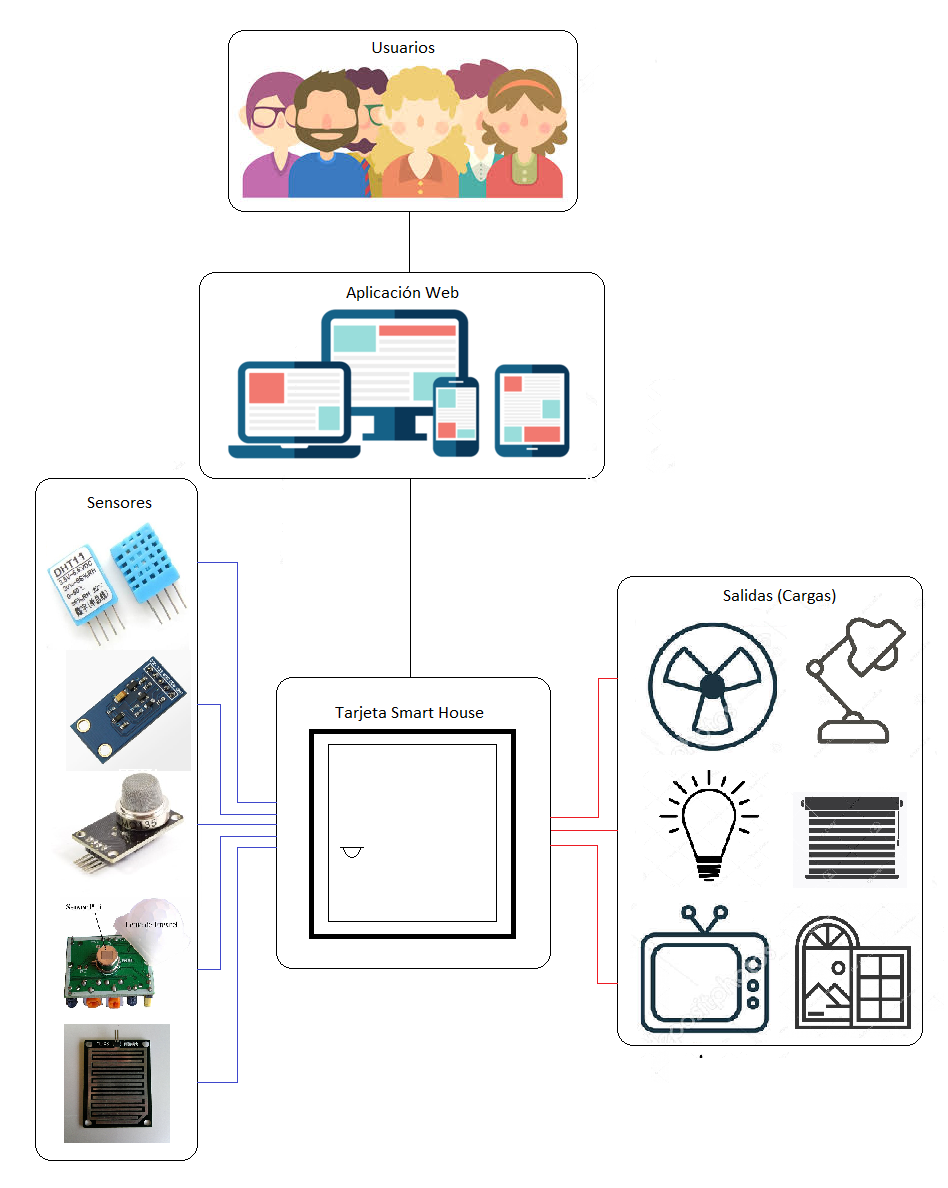
\includegraphics[width=0.7\linewidth]{Imagenes/Diagramas}
	\caption{Esquema del sistema IoT [Imagen Propia]}
	\label{fig:diagramas}
\end{figure}

Para la construcción del hardware se tomaron como referencia valores de operación presentes en el mercado, de modo que las salidas para cargas DC fueron definidas a un voltaje de 12V, ya que se comercializan dispositivos como lámparas LEDs o mecanismos capaces de abrir y cerrar ventanas o persianas con este nivel de tensión, entre otros. Por otra parte, el voltaje para las cargas AC se define con base en la red eléctrica doméstica de Colombia, siendo esta 110VAC. Para las entradas del dispositivo se cuenta con los sensores mencionados anteriormente en la Sección \ref{sec:sensors}, los cuales funcionan con voltajes lógicos de 5V y 3.3V. Estos sensores se eligen por ser los más usados en dicho ámbito además de que se acomodan a las necesidades de una habitación, como sensar presencia, temperatura, calidad del aire y demás.\\

Además, para el funcionamiento del Firmware y el Hardware se hace uso del ESP32 como unidad central de mando, ya que cuenta con un procesador de 32 bits de dos núcleos, de los cuales uno de ellos se encarga de la conexión WiFi, mientras que el otro se encarga de los demás procesos del sistema descritos en el presente capítulo. Adicionalmente, el ESP32 cuenta con múltiples salidas y entradas como DACs y ADCs, lo cual permite manejar salidas de audio, entradas analógicas y demás. La ventaja del ESP32 es su integración del WiFi, Bluetooth y otras capacidades en un solo chip en comparación con las distintas tarjetas presentes en el mercado; también su precio con respecto a las funcionalidades que este ofrece.\\



\section{Hardware}\label{sec:hw}

El prototipo para Smart House tiene por objetivo monitorear el entorno de aplicación y controlarlo por medio de mecanismos como motores o dispositivos de iluminación, razón por la cual está equipada con etapas de potencia de corriente alterna y directa como se muestra en el diagrama de la Figura \ref{fig:tar}, etapa de adquisición de datos, entre otras características que permitan cumplir con los objetivos planteados.\\

\begin{figure}[H]
	\centering
	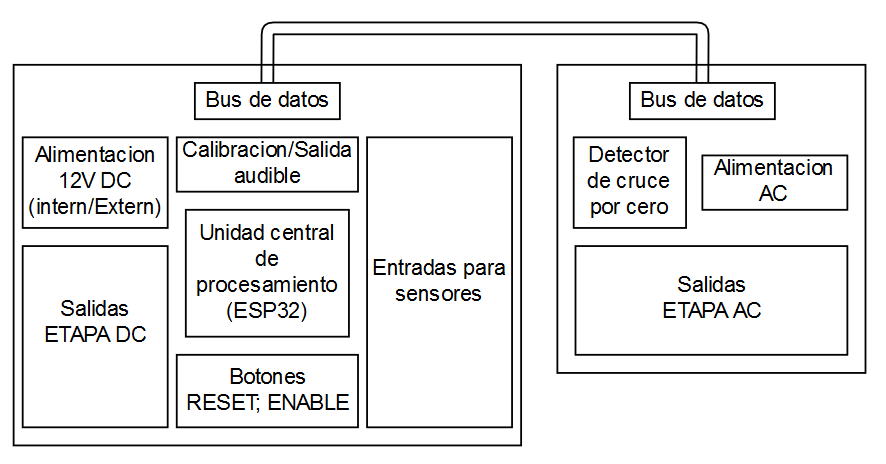
\includegraphics[width=0.7\linewidth]{Imagenes/Tarjeta}
	\caption{Diagrama de la tarjeta Smart House [Imagen Propia]}
	\label{fig:tar}
\end{figure}


El prototipo fue diseñado en el software Proteus, desde el esquemático hasta la placa de circuito impreso (PCB). En la Figura \ref{fig:esp32} se observa el diagrama esquemático de la tarjeta ESP32 construido junto con su distribución de pines, además de sus conexiones correspondientes dentro de este programa. El prototipo está separado en dos secciones, la etapa de potencia AC y la etapa DC, en la última, se encuentra la mayor parte de circuitos que funcionan con corriente directa.\\

\begin{figure}[H]
	\centering
	\caption{ESP32 creado en proteus [Imagen Propia]}
	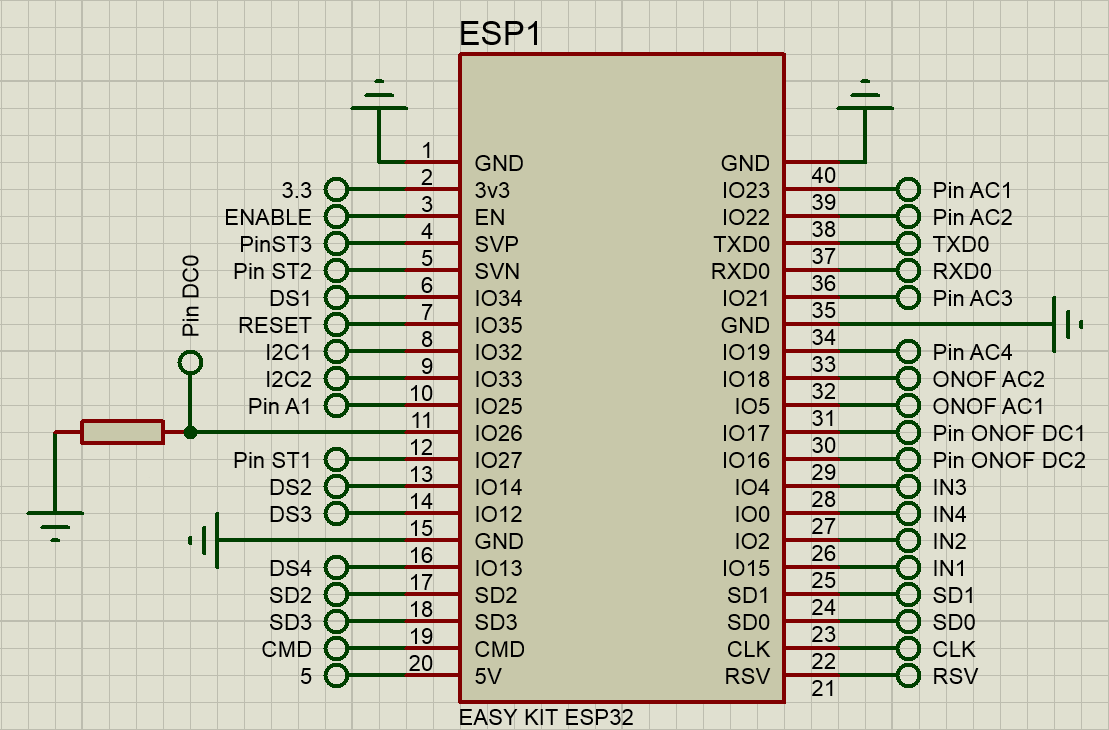
\includegraphics[width=0.5\linewidth]{Imagenes/ESP32}	
	\label{fig:esp32}
\end{figure}

En los siguientes ítems se resaltarán las características más importantes que lleva el circuito:\\

	\subsection{Alimentación}
	
	\paragraph{Corriente alterna (AC):}
		El prototipo recibe el voltaje directamente de la red eléctrica a la que se encuentra conectado el entorno de aplicación, el cual está pensado para una habitación dentro de una Smart House; en el caso de Colombia, la red doméstica comúnmente otorga 110V AC, los cuales son regulados para el funcionamiento adecuado del prototipo, como la etapa de potencia AC y el detector de cruce por cero con el fin de sincronizar la tarjeta a dicha red eléctrica.\\
		
	\paragraph{Corriente directa (DC):}
		Para la alimentación DC del circuito, se hace uso de un conversor AC-DC que regula el voltaje de la red eléctrica a 12V DC, con los cuales se maneja la etapa de potencia DC, además de ser usados por dos módulos conversores DC-DC, mostrados en la Figura \ref{fig:DCDC}, ambos con entradas de 12V DC y con salidas a los niveles lógicos comunes, 5V y 3.3V, empleados con el fin de alimentar dispositivos como optoacopladores, transistores BJT o relevadores con activación de 5V, así como también la tarjeta de prototipo ESP32.\\
		
		Cabe resaltar que la tarjeta permite una entrada externa de 12VDC a 5A si se desean controlar cargas a un máximo de 50W.\\
			
		\begin{figure}[H]
			\centering
			\caption{Módulo conversor DC-DC. Tomado de: \cite{DCDC}}
			\label{fig:DCDC}
			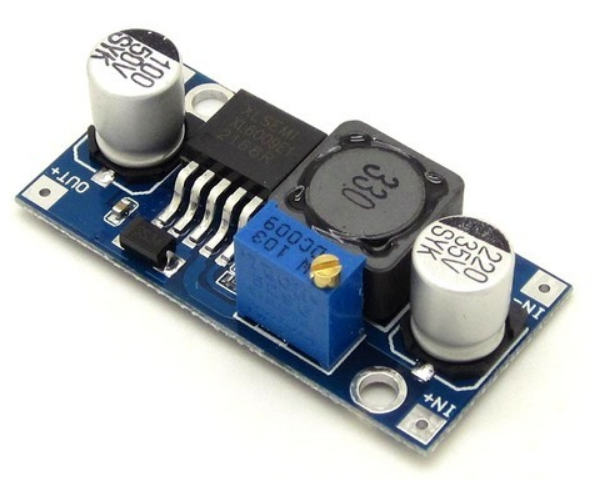
\includegraphics[width=0.5\linewidth]{Imagenes/DCDC}
		\end{figure}
	
	\subsection{Entradas}
	\paragraph{Sensores:}
		El prototipo viene equipado con una etapa de adquisición de datos con capacidad entre 7 a 134 sensores, pues posee una entrada I2C, ampliando el número de dispositivos conectados, lo cual también permitiría adicionar tareas más específicas en escenarios que lo requieran.\\
		
		Con la finalidad de realizar pruebas del prototipo, se hacen uso de 5 sensores para medir magnitudes y situaciones en el entorno, tal como calidad del aire, temperatura, humedad, luz visible, movimiento y presencia de lluvia, debido a que estas medidas o estados se encuentran en casi cualquier ambiente. Teniendo en cuenta que el ESP32 funciona en voltajes lógicos de 3.3V, se tienen 4 entradas de sensores directamente conectados a los pines de la tarjeta, con la capacidad de cambiar el voltaje de alimentación para 3 de ellos, como se muestra en la Figura \ref{fig:SVS}, pues en el mercado se encuentran sensores que manejan voltajes de alimentación ya sea de 3.3V o 5V, mientras que la cuarta entrada se encuentra alimentada con 5V, ya que tiene un uso específico en las pruebas para el sensor de calidad de aire, esta viene acondicionada con un diodo zener en contraposición, para evitar que la tarjeta ESP32 tenga un voltaje de entrada superior a 3.3V, según se observa en la Figura \ref{fig:S1Aire}.\\
		
		Las tres entradas para sensores de estado (ST1, ST2, ST3), a diferencia de las demás, se encuentran conectadas a pines de la tarjeta que no presentan resistencia de pull down por software, por ello se agregan estas al sistema, tal como se observa en la Figura \ref{fig:ST}.\\
		
		\begin{figure}[H]
			\centering
			\caption{Entrada de sensores[Imagen Propia]}
			\label{fig:SVS}
			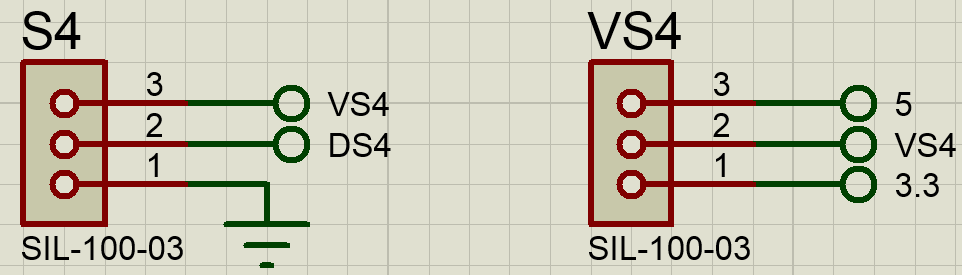
\includegraphics[width=0.7\linewidth]{Imagenes/SVS}
		\end{figure}
	
		\begin{figure}[H]
			\centering
			\caption{Entrada para sensor de calidad de aire[Imagen Propia]}
			\label{fig:S1Aire}
			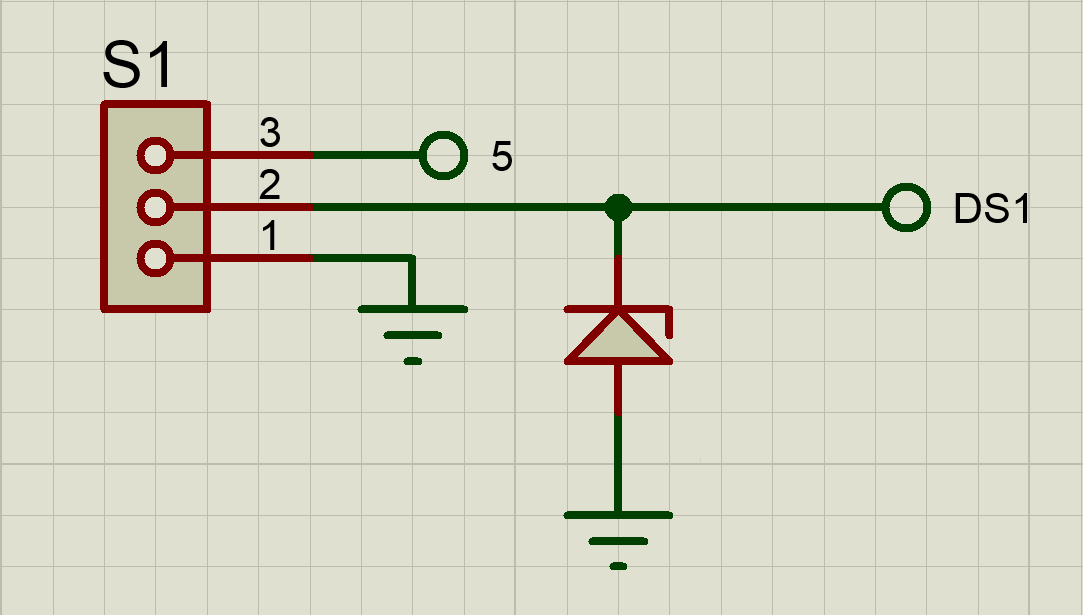
\includegraphics[width=0.6\linewidth]{Imagenes/S1Aire}
		\end{figure}
	
		\begin{figure}[H]
			\centering
			\caption{Entrada para sensores con resistencia de pull down[Imagen Propia]}
			\label{fig:ST}
			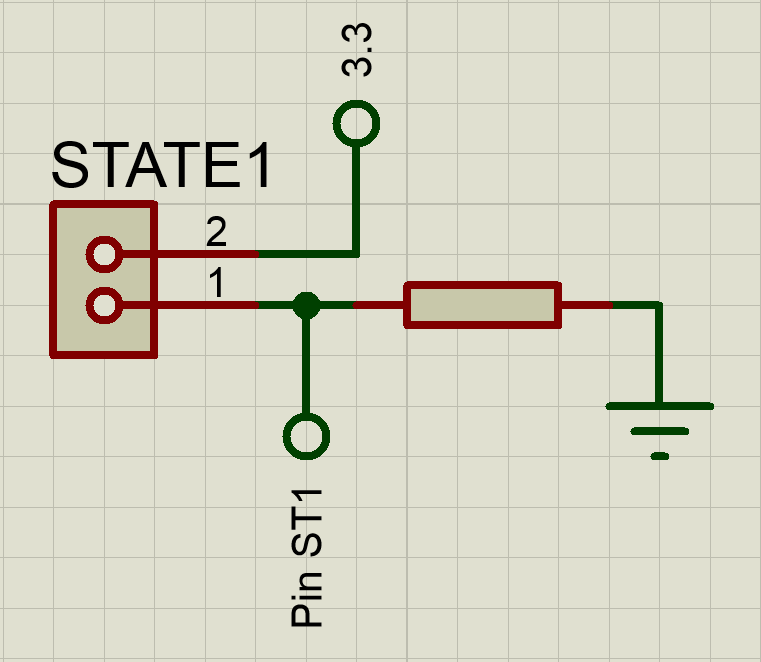
\includegraphics[width=0.5\linewidth]{Imagenes/ST}
		\end{figure}		
	
	\paragraph{Calibración de audio:}
		Para calibrar la salida audible se hace uso de una resistencia variable (Potenciómetro), el cual permite regular el voltaje de entrada al circuito de amplificación mostrado en la Figura \ref{fig:AUD}; este será descrito en el presente capitulo en la sección de salidas del hardware.\\ 
		
	\paragraph{Botón enable:}
		Presionando el botón enable se reinicia la tarjeta ESP32, junto con su firmware.\\
		
	\paragraph{Botón reset:}
		Presionando el botón reset se borran las credenciales ingresadas para la conexión del ESP32 a la red WiFi.\\
		
	\subsection{Salidas:}
	\paragraph{Etapa de potencia AC:}
		Se encuentra diseñada a una potencia de 2000W en un total de seis cargas, cuatro de ellas cuentan con un circuito para el control por ángulo de fase, como se observa en la Figura \ref{fig:CAC1}, con una capacidad individual de 500W, gracias a el TRIAC BTA26600, mostrado en la Figura \ref{fig:TRIAC}, el cual soporta una corriente máxima de 25A. Con el fin de proteger el ESP32, se hace uso de optoacopladores MOC3021, debido a su funcionalidad para aislar circuitos de forma óptica.\\
		
		\begin{figure}[H]
			\centering
			\caption{Control por ángulo de fase [Imagen Propia]}
			\label{fig:CAC1}
			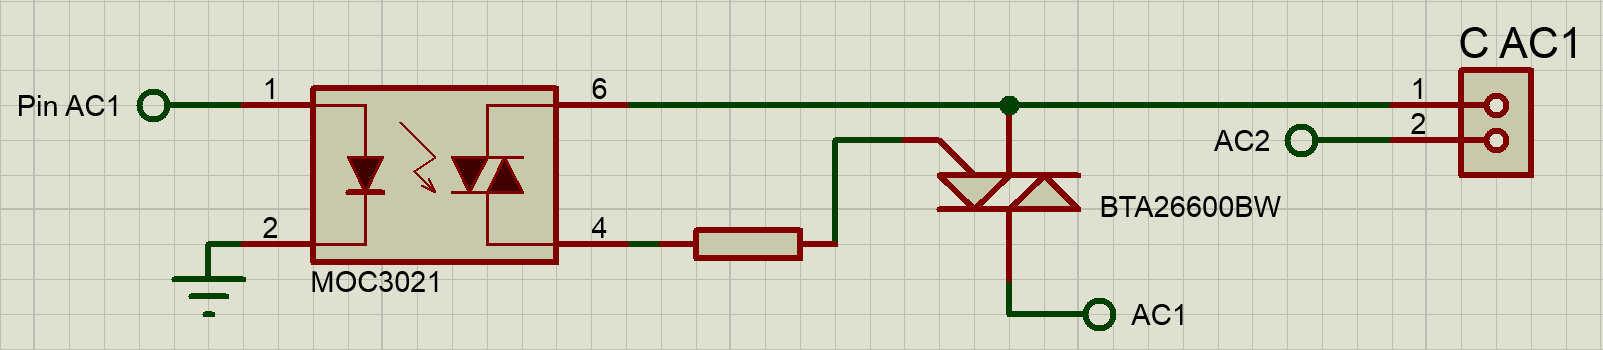
\includegraphics[width=0.8\linewidth]{Imagenes/CAC1}
		\end{figure}
	
		\begin{figure}[H]
			\centering
			\caption{Triac BTA26600. Tomado de: \cite{TRIAC}}
			\label{fig:TRIAC}
			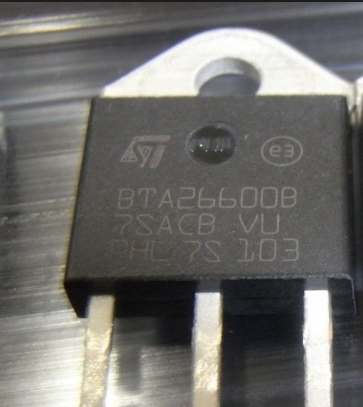
\includegraphics[width=0.35\linewidth]{Imagenes/TRIAC}
		\end{figure}
	
		Las dos cargas restantes corresponden a un sistema de encendido y apagado, cuyo funcionamiento se basa en un relevador SRA-05VDC-CL activado a 5V por medio de un transistor BJT como switch, gracias a este relé, las salidas tienen capacidad de hasta 200W cada una. En la Figura \ref{fig:ONOFAC} se observa el circuito diseñado en Proteus. Para proteger el ESP32, el prototipo se vale de ese dispositivo, puesto que presenta un aislamiento magnético por la naturaleza de su operación.\\
	
		\begin{figure}[H]
			\centering
			\caption{Interruptor para cargas AC [Imagen Propia]}
			\label{fig:ONOFAC}
			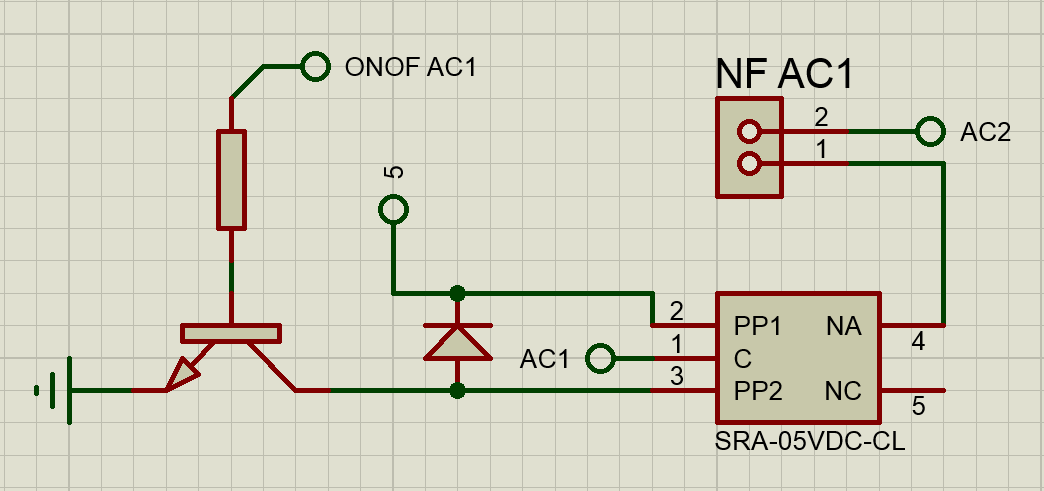
\includegraphics[width=0.7\linewidth]{Imagenes/ONOFAC}
		\end{figure}
	
		Dentro de la etapa AC se encuentra el detector de cruce por cero, el cual cuenta con un fototransistor 4N25, debido a su alta capacidad de aislamiento, tomando la onda rectificada completa y pasándola a un nivel lógico de 3.3V, esta parte del circuito se observa en la Figura \ref{fig:DC01}; para que la señal sea más confiable se hace uso de un Schmitt-Trigger CD40106 mostrado en la Figura \ref{fig:DC02}, valiéndose de la histéresis de voltaje garantizando que la señal de salida sea poco susceptible al ruido \cite{DC0}.\\
		
		\begin{figure}[H]
			\centering
			\caption{Detector de cruce por cero [Imagen Propia]}
			\label{fig:DC01}
			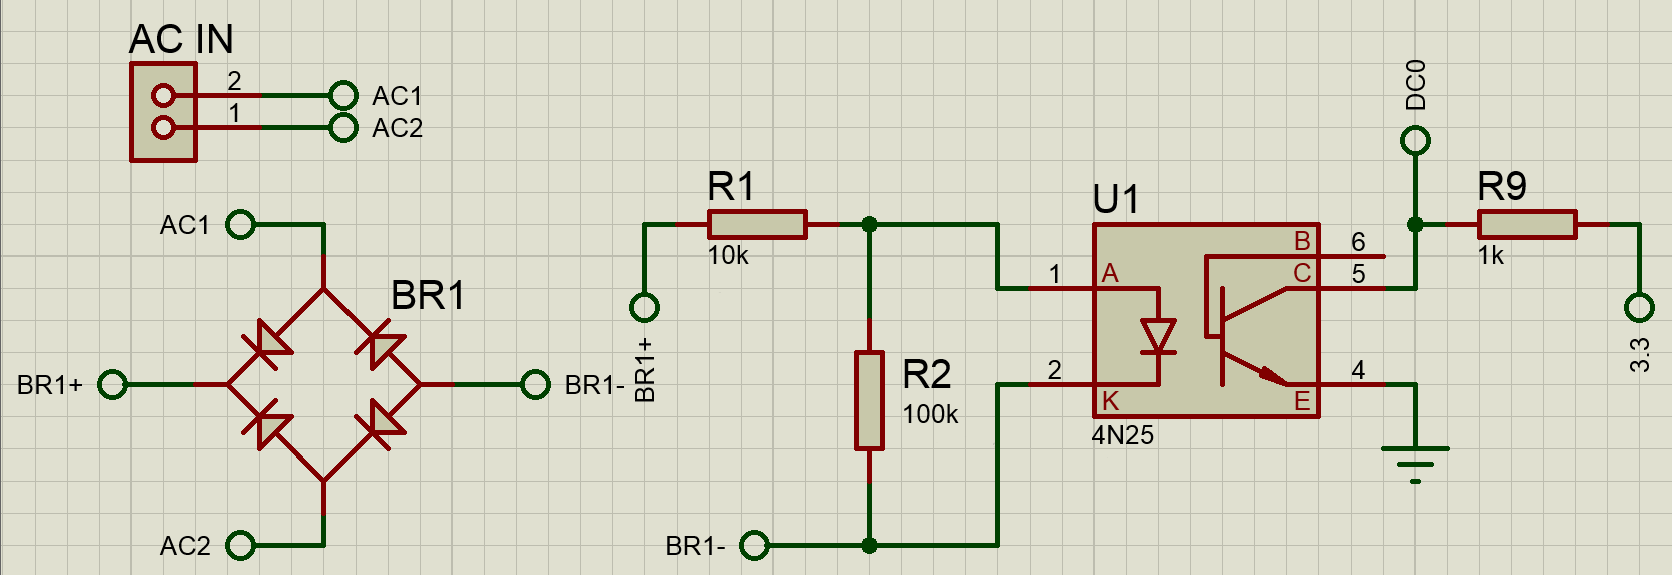
\includegraphics[width=0.85\linewidth]{Imagenes/DC01}
		\end{figure}
	
		\begin{figure}[H]
			\centering
			\caption{Schmitt trigger para el detector de cruce por cero [Imagen Propia]}
			\label{fig:DC02}
			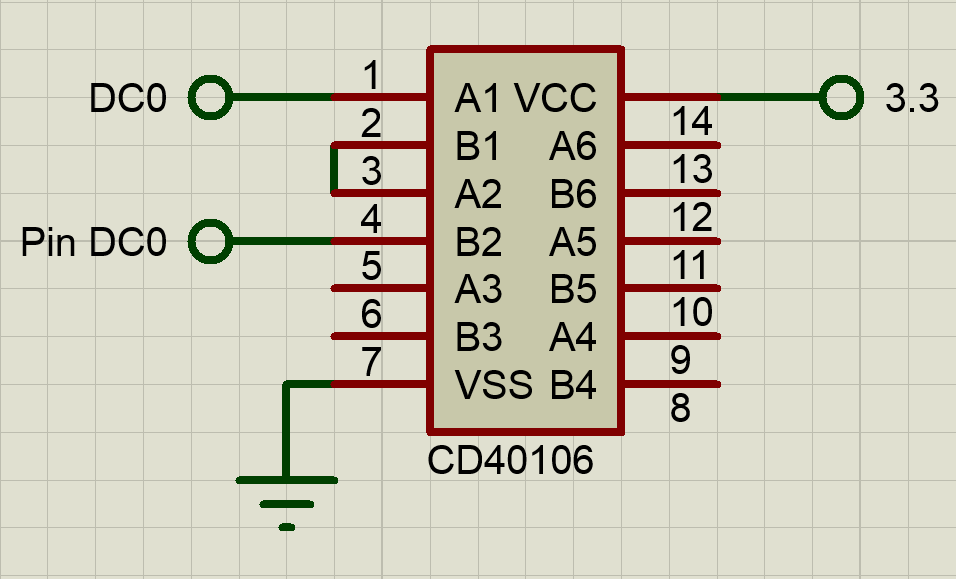
\includegraphics[width=0.5\linewidth]{Imagenes/DC02}
		\end{figure}
	
	\paragraph{Etapa DC:}
		Esta etapa cuenta con cuatro salidas de control diseñadas para cargas de 12V, de las cuales, dos de ellas tienen un enfoque a motores, puesto que está equipada con control de velocidad a base de PWM e inversión de giro con un puente H usando transistores mosfet IRLZ44N; el puente h se encuentra controlado por un circuito integrado L293D, que garantiza un voltaje Vgs adecuado para la correcta activación del los transistores; este circuito se muestra en las Figuras \ref{fig:L293D} y \ref{fig:CDC}.\cite{IRL}.\\
		
		Las dos salidas restantes también cuentan con mosfet IRLZ44N, y su control igualmente es a base de PWM, mas no permite realizar la inversión de giro, por lo cual se enfoca a dispositivos como lámparas LEDs. El diseño en Proteus se muestra en la Figura \ref{fig:ONOFDC}.\\
		
		\begin{figure}[H]
			\centering
			\caption{Integrado L293D [Imagen Propia]}
			\label{fig:L293D}
			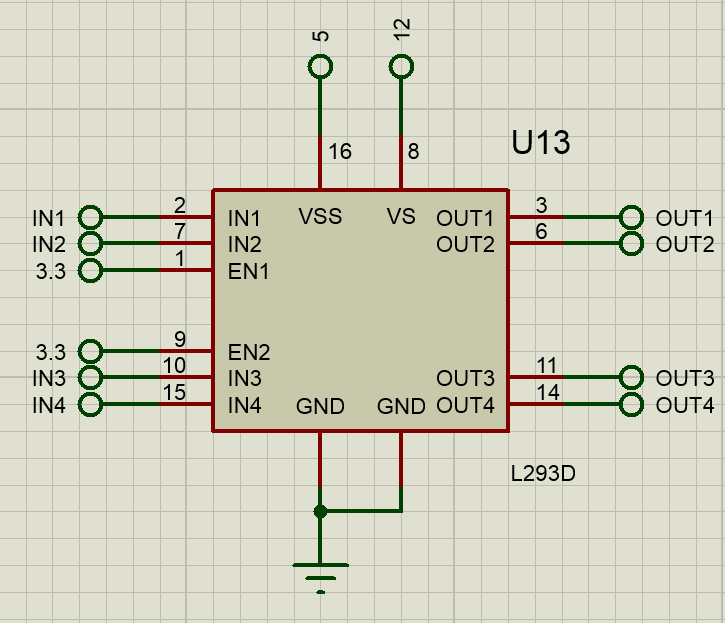
\includegraphics[width=0.5\linewidth]{Imagenes/L293D}
		\end{figure}
		
		\begin{figure}[H]
			\centering
			\caption{Puente H para control de motores DC [Imagen Propia]}
			\label{fig:CDC}
			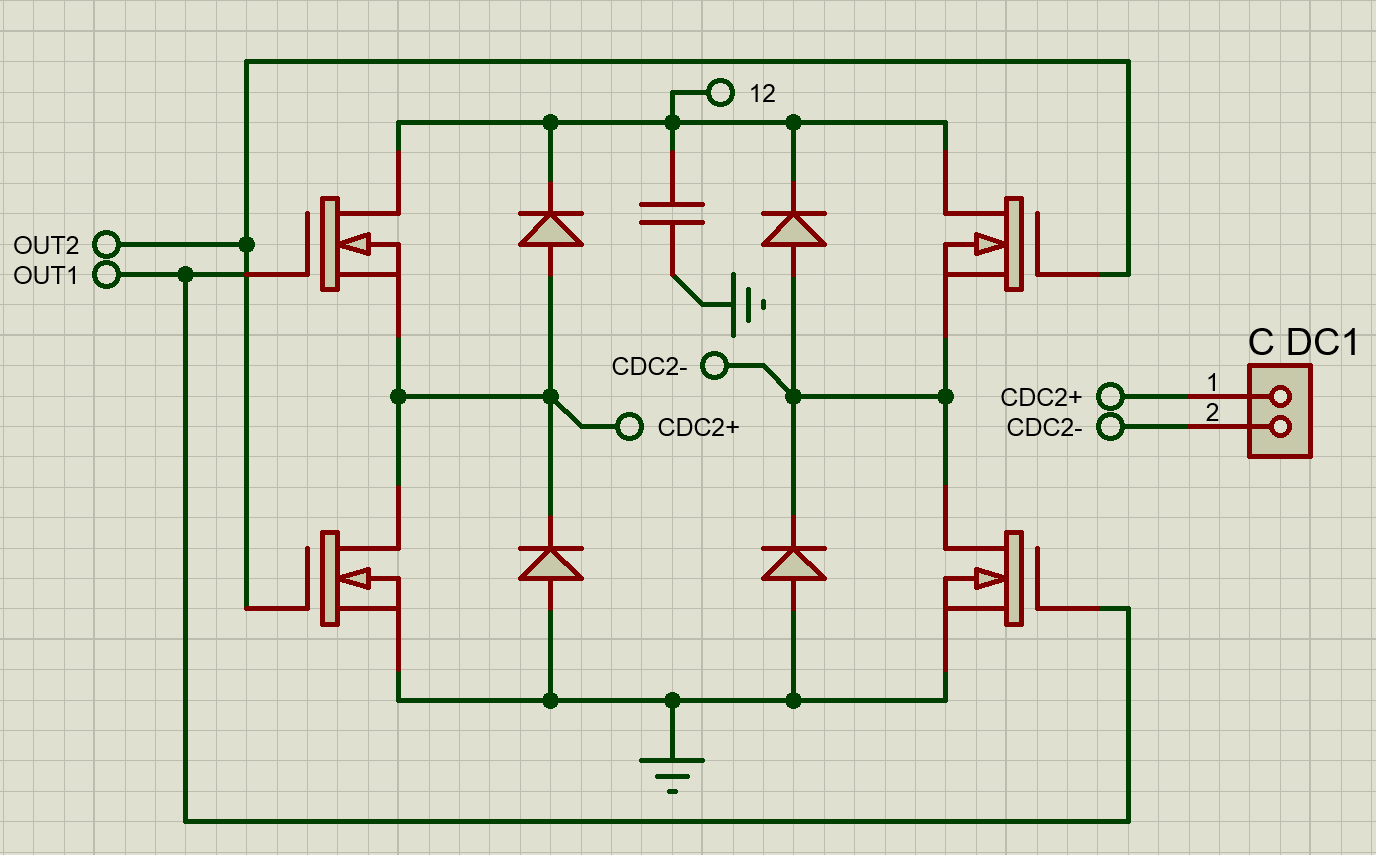
\includegraphics[width=0.7\linewidth]{Imagenes/CDC}
		\end{figure}
	
		\begin{figure}[H]
			\centering
			\caption{Control para cargas DC [Imagen Propia]}
			\label{fig:ONOFDC}
			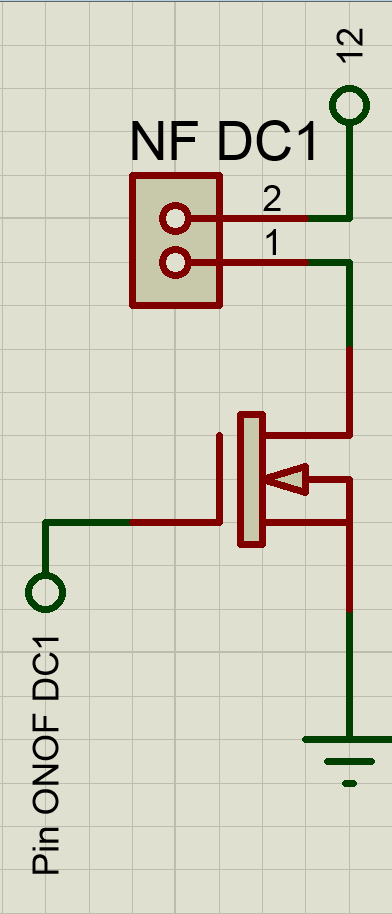
\includegraphics[width=0.25\linewidth]{Imagenes/ONOFDC}
		\end{figure}
	
	\paragraph{Salida audible:}
		Está diseñada para emitir sonidos a una sola frecuencia, o sonido mono estéreo, caso dado cuando se activa una regla programada en la aplicación web, enfocada a las cargas de encendido y apagado, tanto de la etapa de potencia AC como la etapa DC; el sonido emitido por el prototipo corresponde a una voz con tonalidad femenina, pronunciando el estado en el cual se configura la carga según la regla (ya sea encendido, o apagado).\\
		
		El circuito utilizado para la salida audible está basado en el amplificador de audio LM386, implementando el esquema típico de aplicación ilustrado en su datasheet \cite{LM386}. En la Figura \ref{fig:AUD} se observa implementado en el software Proteus.\\
		
		Como se mencionó anteriormente, el circuito presenta un potenciómetro a la entrada para calibrar el voltaje de esta, con el objetivo de no saturarla y que la salida sea lo más fiel posible.\\
		
		\begin{figure}[H]
			\centering
			\caption{Circuito tipico para el LM386 [Imagen Propia]}
			\label{fig:AUD}
			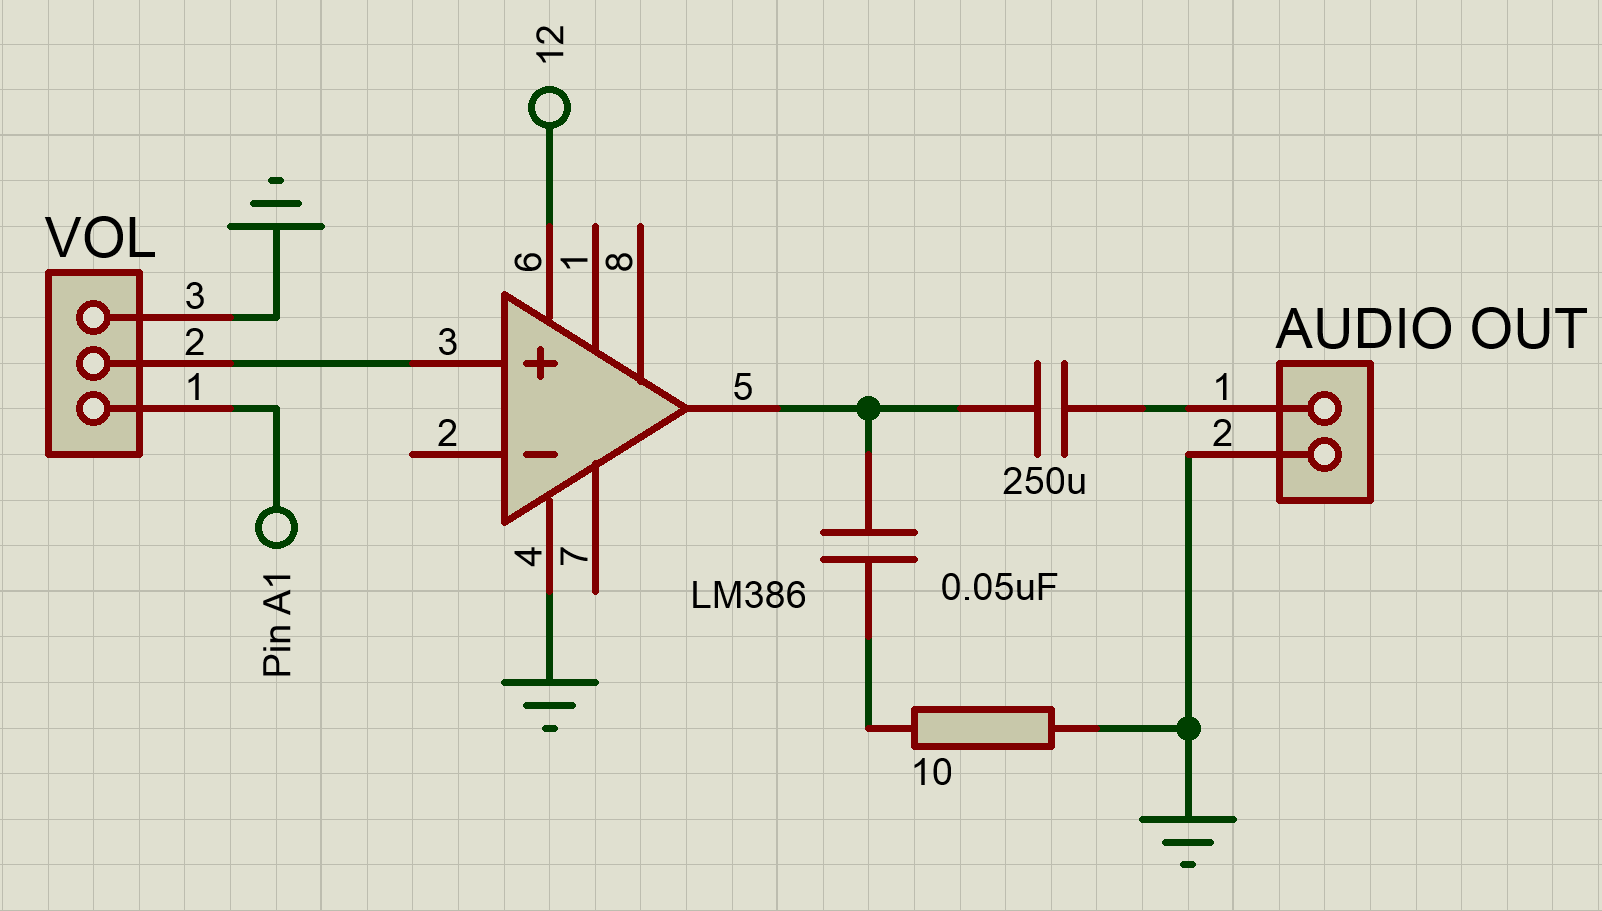
\includegraphics[width=0.7\linewidth]{Imagenes/AUD}
		\end{figure}		
				
\section{Firmware}

El firmware se desarrolla sobre el framework o SDK oficial de Espressif Systems ESP-IDF, el cual posee una documentación \cite{ES} muy útil a la hora de utilizar las diferentes APIs presentes en este; para el desarrollo de la aplicación es necesario contar con los requisitos que se observan en la Figura \ref{fig:what-you-need}. Esta característica del sistema incluye un kernel de tiempo real llamado FreeRTOS, el cual da soporte al manejo de los diversos recursos del sistema; al ser un RTOS, las funciones se definen mediante tareas, entonces cada funcionalidad de la tarjeta o grupo de funcionalidades se desarrolla en una o varias tareas que realicen las acciones adecuadas. Por ejemplo, en el caso de los sensores, cada uno tiene una tarea para la lectura y gestión de datos, así como también ocurre de manera similar con las salidas de la tarjeta, pues cuentan con tareas encargadas de la gestión del encendido y apagado, asimismo para el control de cargas, ya sea por ángulo de fase o PWM.\\

\begin{figure}[H]
	\centering
	\caption{ESP-IDF. Tomado de: \cite{ES}}
	\label{fig:what-you-need}
	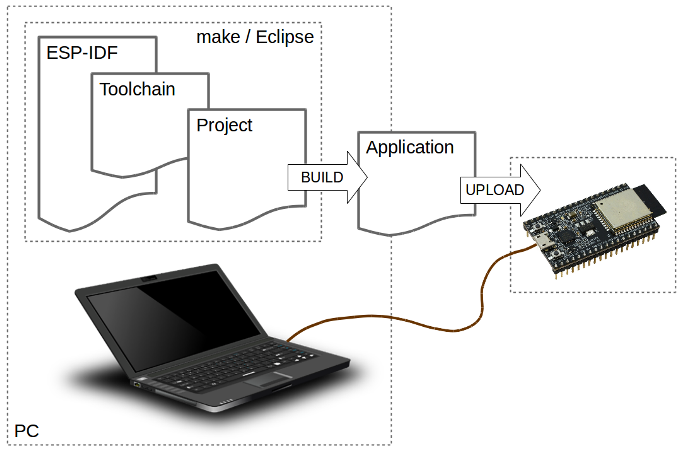
\includegraphics[width=0.5\linewidth]{Imagenes/what-you-need}
\end{figure}


Sobre el firmware se desarrollan los siguientes temas:

\paragraph{Tareas:}

Se ejecutan constantemente en el sistema operativo, realizando diferentes funciones para lectura, escritura y control.

\paragraph{GPIO:}

El ESP-WROOM-32 posee diferentes GPIO, los cuales se usan para leer o escribir señales digitales; en cuanto a los sensores, se pueden enviar señales con el fin de iniciar su lectura o simplemente tener el pin en modo entrada y leerlo cada cierto intervalo de tiempo generando datos de lectura, o en modo salida para el control de los diversos dispositivos que se han desarrollado en el hardware.

\paragraph{ADC,DAC:}

Los ADC se usan para leer los datos de algunos sensores que proporcionan señales analógicos, por este motivo se hace la conversión de la señal analógica a un valor digital dentro de la tarjeta, así luego identificar el dato de la lectura del sensor. Los DAC son usados para realizar la operación contraria, es decir, teniendo valores digitales convertirlos a un valor analógico por ejemplo generar audios o diferentes señales a partir del software.

%\paragraph{Consola:}para realizar diferentes pruebas directamente desde la tarjeta, se usa la opción de la consola, la cual se comunica por medio del puerto serie, para esto se crean las funciones y los comandos que estaran disponibles; algunos son \textit{http}, para ejecutar las peticiones http manualmente y observar su respuesta, \textit{pin} para realizar la prueba de un pin digital como entrada o salida, \textit{help} para observar la lista de comandos, entre otros.

\paragraph{HTTP Request:}

Las peticiones HTTP son indispensables en estas aplicaciones del campo IOT, por tal motivo en el desarrollo del firmware se usan las librerías pertinentes para realizarlas y además leer las respuestas de estas desde el servidor, ya que este es el medio de comunicación tarjeta-servidor.

\paragraph{Hora de Red:}

Se obtiene la hora mediante el protocolo simple de tiempo de red (SNTP), este resulta de gran utilidad para la sincronización de los relojes de los sistemas informáticos. Se mantiene actualizada con el objetivo de realizar diferentes acciones respecto a esta.

\paragraph{Timers:}

La tarjeta posee dos grupos de timers y cada uno tiene dos timers, un timer lo usa el sistema operativo, otro es configurado con el fin de realizar el control de potencia AC por ángulo de fase, para tener la sincronía necesaria con la señal de la red eléctrica.

\paragraph{I2C:}

El protocolo I2C se activa por medio de la instalación del driver en algún par de pines GPIO disponibles en la tarjeta. Se configura e inicia y posteriormente se crea una tarea la cuál se encarga de solicitar y leer los datos de los diferentes sensores conectados a este.

\paragraph{PWM:}

Se ha mencionado anteriormente que con el propósito de controlar las cargas DC se usa una salida PWM, el ESP32 proporciona esta funcionalidad en algunos de sus pines, para su uso se configura y asignan los valores de funcionamiento.

\paragraph{Interrupciones:}

Las interrupciones se usan para no gastar recursos en un monitoreo constante de las entradas, solo cuando exista un cambio de nivel en la entrada el dispositivo desencadena una serie de instrucciones relacionadas con el tipo de interrupción y diversas funciones creadas para esta, la interrupción se usa por medio de los diferentes pines con este propósito en el hardware.

\section{Software}

En esta sección se desarrolla una aplicación web, la cual se encarga de ejecutar la gestión entre el usuario y la tarjeta. De este modo, se usa un patrón de arquitectura Modelo-Vista-Controlador (MVC), siendo este realmente útil ya que separa la lógica de negocio de la interfaz de usuario, incrementando la reutilización y flexibilidad, además de la escalabilidad de ambos aspectos por separado, dicho esto, la aplicación cuenta con diferentes modelos, controladores y vistas \cite{MVC1}. La función de cada parte de esta arquitectura se puede observar en la Figura \ref{fig:mvc}.\\

\begin{figure}[H]
	\centering
	\caption{Modelo-Vista-Controlador [Imagen Propia]}
	\label{fig:mvc}
	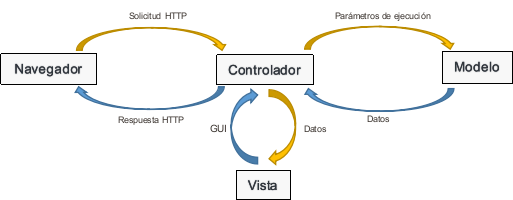
\includegraphics[width=0.7\linewidth]{Imagenes/MVC}
\end{figure}


Su funcionamiento es el siguiente, primero el usuario realiza alguna acción en la interfaz (por ejemplo, presiona un botón, un enlace, etc), luego el controlador recibe (por parte de los objetos de la interfaz-vista) la notificación de la acción solicitada por el usuario. El controlador gestiona el evento que llega, accediendo al modelo y actualizándolo, posiblemente modificándolo de forma adecuada a la acción solicitada por el usuario (por ejemplo, el controlador actualiza los datos del perfil del usuario) y después la interfaz de usuario espera nuevas interacciones del usuario, comenzando el ciclo nuevamente \cite{MVC2}.\\

Este patrón de diseño se usa en la programación orientada a objetos, por lo tanto se realiza la aplicación en el lenguaje de programación PHP, ya que es realmente útil para realizar la gestión de peticiones y envíos de formularios en dicha aplicación, además de que es importante también la gestión de las bases de datos de la aplicación, por este motivo se utiliza un framework basado en este lenguaje y esta arquitectura. Para gestionar las diferentes partes de la aplicación, en este caso se usa el framework Laravel, pues como se menciona anteriormente, está orientado a facilitar las tareas comunes de la mayoría de proyectos web que utilizan HTML5 y PHP.\\

Además, con este framework se hace uso de un ORM (Mapeo Objeto-Relacional) llamado Eloquent. Esta es una forma de mapear los datos que se encuentran en la base de datos a objetos de PHP y viceversa, esto facilita el uso de diferentes gestores de bases de datos como MySQL, SQLite, entre otras, ya que todas las consultas estan en PHP y el ORM ya se encarga del mapeo a los comandos SQL como se observa en la Figura \ref{fig:orm}. Eloquent usa los modelos para enviar y recibir información de la base de datos\cite{Eloq}.\\

\begin{figure}[H]
	\centering
	\caption[ORM]{ORM [Imagen Propia]}
	\label{fig:orm}
	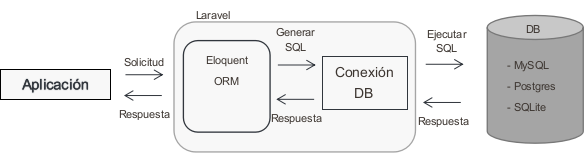
\includegraphics[width=0.7\linewidth]{Imagenes/ORM}
\end{figure}

\section{Prueba Beta}

Esta prueba se desarrolla en el entorno del cliente o usuario, arrojando resultados sobre las funcionalidades provistas para el software, además de dar la aceptación por parte del cliente si el producto funciona de manera adecuada o esperada \cite{PB}. Con el fin de realizar dicha verificación se analizan los objetivos a cumplir y los alcances, por lo tanto se separan los casos de prueba con el propósito de formular las preguntas que deben contestar las personas.\\

En general se ha propuesto el desarrollo de una solución IoT, con alcances como controlar cargas AC o DC y visualizar el estado del entorno de aplicación por medio de la página web desarrollada, además de que esta aplicación web sea fácil de usar para el usuario, por este motivo se presentan los diferentes casos de prueba a realizar y se mencionan a continuación; las preguntas formuladas para estos se encuentran en el Anexo \ref{AnexoB}.

\paragraph{Prueba de conectividad de la tarjeta:} La persona que participa en esta prueba debe realizar los primeros pasos para conectar la tarjeta con internet como se expone más adelante en resultados y se explica en Anexos en el manual de usuario.\\

De acuerdo con esto se califica la forma en que el cliente realiza este procedimiento, con la finalidad de analizar si es adecuada la manera en que se conecta la tarjeta SmartHouse a Internet por medio de Wi-Fi y también como reiniciar la conexión de la tarjeta para configurar nuevamente la red a la que se va a conectar. Las preguntas del número uno a la tres califican esta funcionalidad.\\

\paragraph{Prueba de la Aplicación Web:} Evalúa el inicio de sesión, el monitoreo y control de todos los dispositivos que se encuentra conectados en tarjeta SmartHouse, además de las funcionalidades que posee el sistema en general.\\

Para esta prueba se deben realizar diferentes procedimientos, como iniciar sesión en la aplicación, encender o apagar un dispositivo, visualizar los datos de los sensores y configurar las reglas para los dispositivos. Las preguntas presentes en el Anexo \ref{AnexoB} de la número cuatro en adelante califican estos aspectos y funcionalidades.\\